\section{A Tree Representation of Subinstances}
In this section we discuss how to represent all subinstances of some arbitrary
instance $\mathcal{Q}$. We also discuss how to identify 
subinstances to which we do not already know the solution.
We construct a \emph{tree} of all subinstances with distinct optimal solutions.
This tree enables us to efficiently check whether some modifier forms a
subinstance with an unknown solution.

If we were to try to solve all $u$ possible subinstances of an
instance, we would most likely end up solving a huge amount of subinstances
with the same optimal solutions. This is evident in some of the real
instances; when we solve the unmodified instance \texttt{vlarge}, if $b = n$,
we already have the solution to $2^{1749}$ of its possible subinstances, i.e.
$|\mathcal{Z}_0| = 1749$.
Just trying to unnecessarily solve all these subinstances---let alone store the
solutions---would be a huge waste of resources.
Instead, we try to identify subinstances with distinct optimal solutions.
A good starting point is to find all the subsets of $\mathcal{N}_0$ and
use them as modifiers of $Q$. This is equivalent to forcing non-zero
variables in the optimal solution of the unchanged instance $Q$, to zero.
Recall from the previous section that if $\mathcal{Q}$ is known, knowing the
modifier $\mathcal{M}_k$ is sufficient to identify the subinstance
$\mathcal{Q}_k$.
While finding modifiers $\mathcal{M}_k$ such that
$\mathcal{M}_k \subseteq \mathcal{N}_0$ ensures that $x_k^*\neq x_0^*$,
it does not assure us that $x_k^* \neq x_l^*$ for all $l=1,2,\ldots,u-1$.
To make sure that we only solve subinstances with distinct optimal solutions,
we need to identify modifiers $\mathcal{M}_k$ such that
$\mathcal{M}_k \not \subset \mathcal{Z}_l$
for \emph{all} $l=1,2,\ldots,u-1$.

Consider a set $\mathbb{U}\subseteq \left\{{1,2,\ldots,u-1}\right\}$ of indices
such that if $i,j \in \mathbb{U}$, and $i \neq j$, then $x_i^* \neq x_j^*$.
With such a set; given an arbitrary modifier $\mathcal{M}_k$, we can check
if there exists an index $l \in \mathbb{U}$ such that $x_k^* = x_l^*$. By
checking each index $i \in \mathbb{U}$, we only need to confirm that
$\mathcal{M}_k \subseteq \mathcal{Z}_i$ to know that $x_k^* = x_i^*$. However,
checking each element of $\mathbb{U}$ might not be practical when the set
grows large. With a tree representation of $\mathbb{U}$, we can (dis)confirm
that $x_k^* = x_l^*$ for a modifier $\mathcal{M}_k$ without checking \emph{all}
indices in the set.

%To make sure that we do not solve any unnecessary subinstances, we need
%find modifiers $\mathcal{M}_k$ such that
%$\mathcal{M}_k \not \subset \mathcal{Z}_l$
%for \emph{all} $l=1,2,\ldots,2^n-1$.

%Consider a set $\mathbb{U}$ that contains all subinstances $\mathcal{Q}_k$
%such that $x_k^* \neq x_l^*$ for all
%$\mathcal{Q}_l \in \mathbb{U} \backslash \mathcal{Q}_k$.
%While constructing such a set, we have to obey the following rule:
%If $\mathcal{M}_k$ is a subset of any $\mathcal{Z}_l \in \mathbb{U}$, we know
%that $x_k^* = x_l^*$ and therefore we do not add $\mathcal{Q}_k$ to
%$\mathbb{U}$;
%if however, the opposite is true, we add $\mathcal{Q}_k$ to $\mathbb{U}$.
%With such a set; given an arbitrary modifier $\mathcal{M}_k$, we could check
%whether we would need to solve its corresponding subinstance $\mathcal{Q}_k$ or
%not.
%The downside is that we need to check all elements in $\mathbb{U}$ for
%each modifier we want to check.
%By constructing a tree instead of a set, we could check a modifier without
%checking it against all previous subinstances we have solved.

We define a tree as an ordered pair $G = (V,E)$ comprising a set $V$ of
vertices together with a set $E$ of edges.
Let each vertex $v_k \in V$ represent an index $k \in \mathbb{U}$.
For each vertex $v_k$ and its parent $v_l$, $\mathcal{M}_l$ must
be a subset of $\mathcal{M}_k$.
Put differently, each vertex and its corresponding modifier in the tree must be
an extension of the modifier of its parent.
The root $v_0$, which does not have a parent, has a modifier that is equal
to the empty set, i.e. $\mathcal{M}_0 = \emptyset$.

\begin{algorithm}[h!]
\caption{\texttt{find($\mathcal{M}_l$, $v_k$)}}
\label{alg:find}
%\KwIn{($\mathcal{M}_l$, $\mathcal{Q}_k$)}
\SetAlgoVlined
\ForEach{child vertex $v_i$ of $v_k$}{
  \If{$\mathcal{M}_i \subseteq \mathcal{M}_l$}{
    \eIf{$\mathcal{M}_l \subseteq \mathcal{Z}_i$}{
      \textbf{return} $i$
%      \KwRet{$i$}
    }{
      \texttt{find($\mathcal{M}_l$, $v_i$)}
%      \KwRet{find($\mathcal{M}_l$, $v_i$)}
    }
  }
}
\KwRet{$-1$}
\end{algorithm}


Algorithm \ref{alg:find} describes an algorithm for finding the index
$i \in \mathbb{U}$ for a given modifier $\mathcal{M}_l$ such that
$x_l^* = x_i^*$.
Note that the return value
on the last line of the algorithm is implementation specific, but it should be
a value that somehow tells us that we have not previously found the solution to
$\mathcal{Q}_l$.

Consider a tree $G$ with a vertex set $V = \left\{{v_0,v_1,\ldots,v_{10}}\right\}$
and an edge set $E = \left\{{\left\{{0,1}\right\},\left\{{0,2}\right\},\left\{{0,3}\right\},\left\{{0,4}\right\},\left\{{1,5}\right\},\left\{{2,6}\right\},\left\{{4,7}\right\},\left\{{5,8}\right\},\left\{{6,9}\right\},\left\{{9,10}\right\}}\right\}$
and the following values:
\[
    \begin{array}{ll}
        \mathcal{M}_0 = \left\{{}\right\}           & \mathcal{Z}_0 = \left\{{1,3}\right\} \\
        \mathcal{M}_1 = \left\{{2}\right\}          & \mathcal{Z}_1 = \left\{{2,3,5}\right\} \\
        \mathcal{M}_2 = \left\{{4}\right\}          & \mathcal{Z}_2 = \left\{{4,1,5}\right\} \\
        \mathcal{M}_3 = \left\{{5}\right\}          & \mathcal{Z}_3 = \left\{{5,1,3}\right\} \\
        \mathcal{M}_4 = \left\{{2,4}\right\}        & \mathcal{Z}_4 = \left\{{2,4,3,5}\right\} \\
        \mathcal{M}_5 = \left\{{2,1}\right\}        & \mathcal{Z}_5 = \left\{{2,1,4,5}\right\}
    \end{array}
    \begin{array}{ll}
        \mathcal{M}_6 = \left\{{4,3}\right\}        & \mathcal{Z}_6 = \left\{{4,3,1}\right\} \\
        \mathcal{M}_7 = \left\{{2,4,1}\right\}      & \mathcal{Z}_7 = \left\{{2,4,1,3}\right\} \\
        \mathcal{M}_8 = \left\{{2,1,3}\right\}      & \mathcal{Z}_8 = \left\{{2,1,3,5}\right\} \\
        \mathcal{M}_9 = \left\{{4,3,5}\right\}      & \mathcal{Z}_9 = \left\{{4,3,5,2}\right\} \\
        \mathcal{M}_{10} = \left\{{4,3,5,1}\right\} & \mathcal{Z}_{10} = \left\{{4,3,5,1,2}\right\} \\
    \end{array}
\]
The tree $G$ is a tree representation of a set $\mathbb{U}$ of some
$\mathcal{Q}$ with $5$ variables.
Figure \ref{fig:find} shows how Algorithm \ref{alg:find} would work with input
$(\left\{{1,2,3,4}\right\}, v_0)$. The left side of the figure shows the tree
specified above. See Appendix \ref{app:tree} for an alternative representation
of the tree.

\begin{figure}[H]
    \centering
    \begin{tabular}[t]{|c|l|}\hline
    \begin{subfigure}[b]{0.35\textwidth}
        \centering
        \input{include/maptreesets2}
    \end{subfigure}
    & 
    \begin{subfigure}[b]{0.64\textwidth}
        \textbf{Finding $\mathcal{M}_l = \left\{{1,2,3,4}\right\}$ from $v_0$} \\
        \begin{tabular}{rll}
            $k$ & $\mathcal{M}_k$            & $\mathcal{Z}_k$ \\ \hline
            0        & $\left\{{}\right\}$        & $\left\{{1,3}\right\}$ \\ 
            1        & $\left\{{2}\right\}$       & $\left\{{2,3,5}\right\}$ \\ 
            2        & $\left\{{4}\right\}$       & $\left\{{4,1,5}\right\}$ \\ 
            3        & $\left\{{5}\right\}$       & $\left\{{5,1,3}\right\}$ \\ 
            4        & $\left\{{2,4}\right\}$     & $\left\{{2,4,3,5}\right\}$ \\ 
        \end{tabular}
%        \\

        We see that $\mathcal{M}_3 \not \subseteq \mathcal{M}_l$, so we ignore
        the subtree of $v_3$ completely. However, $\mathcal{M}_1 \cup
        \mathcal{M}_2 \cup \mathcal{M}_4 \subseteq \mathcal{M}_l$, so we
        continue searching from the vertices $v_1$, $v_2$ and $v_4$.
%        We see that $\mathcal{M}_1$, $\mathcal{M}_2$ and $\mathcal{M}_4$ are
%        subsets of $\mathcal{M}_l$. However, $\mathcal{M}_l$ is not a subset
%        of any of $\mathcal{Z}_1$, $\mathcal{Z}_2$ or $\mathcal{Z}_4$.
%        Therefore we continue the search from the vertices $v_1$, $v_2$,
%        and $v_4$.
    \end{subfigure}
    \\ \hline
    \begin{subfigure}[b]{0.35\textwidth}
        \centering
        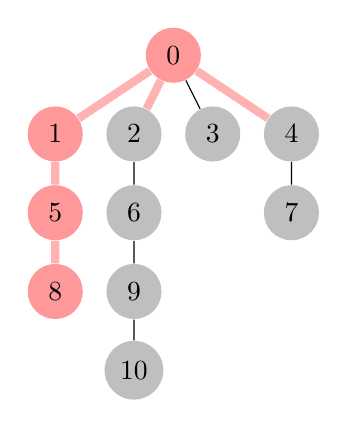
\begin{tikzpicture}[level/.style={sibling distance=10mm/#1, level distance=10mm}]
\tikzset{every node/.style={shape=circle,fill=black!25,minimum size=7mm}}
%\tikzset{every node/.style={shape=circle,
%                            font=\bfseries \Large,
%                            minimum size=3cm,
%                            scale=0.4
%                           }}
\node[fill=red!40] (root) {$0$}
    child {
        node[fill=red!40] {$1$}
        child {
            node[fill=red!40] {$5$}
            child {
                node[fill=red!40] {$8$
                };
                \path edge from parent[draw,line width=3pt,-,red!30];
            };
        \path edge from parent[draw,line width=3pt,-,red!30];
        };
    \path edge from parent[draw,line width=3pt,-,red!30];
    }
    child {
        node {$2$}
        child {
            node {$6$}
            child {
                node {$9$}
                child {node {$10$}
                }
            }
        };
    \path edge from parent[draw,line width=3pt,-,red!30];
    }
    child {node {$3$}}
    child {
        node {$4$}
        child {
            node {$7$}
        };
    \path edge from parent[draw,line width=3pt,-,red!30];
    }
    ;
\end{tikzpicture}

    \end{subfigure}
    & 
    \begin{subfigure}[b]{0.64\textwidth}
        \textbf{Finding $\mathcal{M}_l = \left\{{1,2,3,4}\right\}$ from $v_1$} \\
        \begin{tabular}{rll}
            $k$ & $\mathcal{M}_k$            & $\mathcal{Z}_k$ \\ \hline
            5        & $\left\{{2,1}\right\}$     & $\left\{{2,1,4,5}\right\}$ \\ 
            8        & $\left\{{2,1,3}\right\}$   & $\left\{{2,1,3,5}\right\}$ \\ 
        \end{tabular}
%        \\

        Since $\mathcal{M}_5 \subseteq \mathcal{M}_l \not \subset
        \mathcal{Z}_5$, we continue searching. Continuing, we see that
        $\mathcal{M}_8 \subseteq \mathcal{M}_l \not \subset \mathcal{Z}_8$.
        We would continue the search, but since $v_8$ does not have any child
        vertices, we stop the search and conclude that the subtree of $v_1$
        does not contain a solution for $\mathcal{Q}_l$.
        \\
%        Since $\mathcal{M}_5$ is a subset of $\mathcal{M}_l$ and that
%        $\mathcal{M}_l$ is not a subset of $\mathcal{Z}_5$, we continue
%        searching. Continuing, we see that $\mathcal{M}_8$ is a subset of
%        $\mathcal{M}_l$ and that $\mathcal{M}_l$ is not a subset of
%        $\mathcal{M}_8$. We would continue the search, but since
%        $v_8$ does not have any child vertices, we stop the search
%        and conclude that the subtree of $v_1$ does not contain
%        a solution for $\mathcal{Q}_l$.
    \end{subfigure}
    \\ \hline
    \begin{subfigure}[b]{0.35\textwidth}
        \centering
        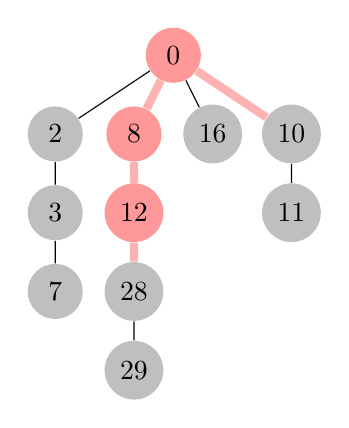
\begin{tikzpicture}[level/.style={sibling distance=10mm/#1, level distance=10mm}]
\tikzset{every node/.style={shape=circle,fill=black!25,minimum size=7mm}}
%\tikzset{every node/.style={shape=circle,
%                            font=\bfseries \Large,
%                            minimum size=3cm,
%                            scale=0.4
%                           }}
\node[fill=red!40] (root) {$0$}
    child {
        node {$2$}
        child {
            node {$3$}
            child {
                node {$7$
                }
            }
        }
    }
    child[fill=red!40] {
        node[fill=red!40] {$8$}
        child {
            node[fill=red!40] {$12$}
            child {
                node {$28$}
                child {node {$29$}
                };
                \path edge from parent[draw,line width=3pt,-,red!30];
            };
            \path edge from parent[draw,line width=3pt,-,red!30];
        };
    \path edge from parent[draw,line width=3pt,-,red!30];
    }
    child {node {$16$}}
    child {
        node {$10$}
        child {
            node {$11$}
        };
    \path edge from parent[draw,line width=3pt,-,red!30];
    }
    ;
\end{tikzpicture}

    \end{subfigure}
    & 
    \begin{subfigure}[b]{0.64\textwidth}
        \textbf{Finding $\mathcal{M}_l = \left\{{1,2,3,4}\right\}$ from $v_2$.} \\
        \begin{tabular}{rll}
            $k$ & $\mathcal{M}_k$            & $\mathcal{Z}_k$ \\ \hline
            6        & $\left\{{4,3}\right\}$     & $\left\{{4,3,1}\right\}$ \\ 
            9        & $\left\{{4,3,5}\right\}$   & $\left\{{4,3,5,2}\right\}$ \\ 
        \end{tabular}
%        \\

        Since $\mathcal{M}_6 \subseteq \mathcal{M}_l \not \subset
        \mathcal{Z}_6$, we continue searching. Continuing, we see that
        $\mathcal{M}_9 \not \subseteq \mathcal{M}_l$ and therefore conclude
        that the subtree of $v_2$ does not contain the solution for
        $\mathcal{Q}_l$.
        \\
%
%        Since $\mathcal{M}_6$ is a subset of $\mathcal{M}_l$ and that
%        $\mathcal{M}_l$ is not a subset of $\mathcal{Z}_6$, we continue
%        searching. Continuing, we see that $\mathcal{M}_9$ is \emph{not} a
%        subset of $\mathcal{M}_l$ and therefore conclude that the subtree of
%        $v_2$ does not contain a solution for $\mathcal{Q}_l$.
        \\
        \\
    \end{subfigure}
    \\ \hline
    \begin{subfigure}[b]{0.35\textwidth}
        \centering
        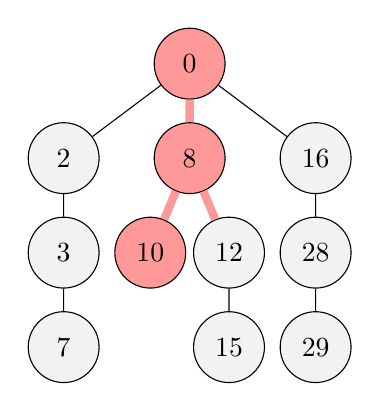
\begin{tikzpicture}
[level 1/.style={sibling distance=16mm, level distance=12mm},
level 2/.style={sibling distance=10mm, level distance=12mm}
]
\tikzset{every node/.style={shape=circle,draw,fill=black!5,minimum size=9mm}}
%\tikzset{every node/.style={shape=circle,
%                            font=\bfseries \Large,
%                            minimum size=3cm,
%                            scale=0.4
%                           }}
\node[fill=red!40] (root) {$0$}
    child {
        node {$2$}
        child {
            node {$3$}
            child {
                node {$7$}
            }
        }
    }
    child {
        node[fill=red!40] {$8$}
        child {
            node[fill=red!40] {$10$};
            \path edge from parent[draw,line width=3pt,-,red!40];
        }
        child {
            node {$12$}
            child {
                node {$15$}
            };
            \path edge from parent[draw,line width=3pt,-,red!40];
        };
    \path edge from parent[draw,line width=3pt,-,red!40];
    }
    child {
        node {$16$}
        child {
            node {$28$}
            child {
                node {$29$}
            }
        }
    }
    ;
\end{tikzpicture}

    \end{subfigure}
    & 
    \begin{subfigure}[b]{0.64\textwidth}
        \textbf{Finding $\mathcal{M}_l = \left\{{1,2,3,4}\right\}$ from $v_4$.} \\
        \begin{tabular}{rll}
            $k$ & $\mathcal{M}_k$            & $\mathcal{Z}_k$ \\ \hline
            7        & $\left\{{2,4,1}\right\}$   & $\left\{{2,4,1,3}\right\}$ \\ 
        \end{tabular}
%        \\

        Since $\mathcal{M}_7 \subseteq \mathcal{M}_l \subseteq \mathcal{Z}_7$
        we conclude that $x_l^* = x_7^*$.
%        Since $\mathcal{M}_7$ is a subset of $\mathcal{M}_l$ and that
%        $\mathcal{M}_l$ is a subset of $\mathcal{Z}_7$ we conclude that
%        $x_l^* = x_7^*$.
        \\
        \\
        \\
        \\
        \\
        \\
        \\
    \end{subfigure}
    \\ \hline
    \end{tabular}
    \caption{\texttt{find} being executed on $G$ where
             $\mathcal{M}_l = \left\{{1,2,3,4}\right\}$.}
    \label{fig:find}
\end{figure}
